\documentclass[hf]{ceurart}

\usepackage{hyperref}
\usepackage{subfigure}
\usepackage{float}
\usepackage{minted}
\usepackage{longtable}
\usepackage{booktabs}
\usepackage{graphicx}
\renewcommand{\thefigure}{\arabic{section}.\arabic{subsection}.\arabic{figure}}
\usepackage[T1]{fontenc}
\usepackage{lmodern}
\setminted{breaklines=true}
\pagenumbering{gobble}
 \pagestyle{empty}
\usepackage{listings}

\usepackage{ntheorem}
\theoremstyle{empty}
\theoremheaderfont{\bfseries\upshape} 
\theorembodyfont{\itshape}
\setlength{\labelsep}{0pt}
\newtheorem{named}{}

\theoremstyle{emptybreak}
\newtheorem{namedbreak}{}


\begin{document}

\makeatletter

\newlength\oriarrayrulewidth  
\newcount\orilowpenalty
\newcommand\nobreakmidrule{%
 \noalign{\global\oriarrayrulewidth\arrayrulewidth\relax
          \global\orilowpenalty\@lowpenalty\relax  
          \global\@lowpenalty=\numexpr-10000\relax%
          \global\arrayrulewidth\lightrulewidth\relax}
 \hline
 \noalign{\global\@lowpenalty=\orilowpenalty\relax%
          \global\arrayrulewidth\oriarrayrulewidth\relax}}

\makeatother
%%
%% Rights management information.
%% CC-BY is default license.
\copyrightyear{2024}
\copyrightclause{Copyright for this paper by its authors.
  Use permitted under Creative Commons License Attribution 4.0
  International (CC BY 4.0).}

\conference{The Tenth Joint Ontology Workshops (JOWO’24), July 15-19, 2024, Enschede, Netherlands}

%% old: \title{Competence Questions in the context of energy systems analysis}
\title{A battery electric vehicle charging infrastructure ontology for interdisciplinary research}

\author[1]{{Eugenio Salvador} {Arellano Ruiz}}[%
orcid=0000-0003-2508-3976,
email=eugenio.arellanoruiz@dlr.de]
\author[1]{Fabia Miorelli}[%
orcid=0000-0001-5095-5401,
email=fabia.miorelli@dlr.de]
\author[1]{Niklas Wulff}[%
orcid=0000-0002-4659-6984,
email=niklas.wulff@dlr.de]
\author[1]{Carsten Hoyer-Klick}[%
email=carsten.hoyer-klick@dlr.de]


\address[1]{German Aerospace Center (DLR), Department of Energy Systems Analysis, Institute of Networked
	Energy Systems, Stuttgart, Germany}


\begin{abstract}
Multidiscipline analyses are prone to misunderstandings associated with rich
discipline-specific semantics. The research of low carbon energy systems is an
example of such applications where concepts coming from multiple expert groups
collide. One very relevant example is the transport-energy nexus where
`sector-coupling' analyses are performed. In this context battery electric
vehicle (BEV) charging infrastructure comprises a main point of interaction for
both research disciplines. Ontologies like the Open Energy Ontology (OEO) where
conceived to aid in the concretization of agreement in such multidisciplinary
research. But since it is a tool whose focus is  energy systems research, it falls
short in concepts associated with transport research. In this paper we propose
a FAIR Ontology, which should work as a first interoperability layer between
the OEO and other ontologies intending to represent concepts associated with
BEV Charging Infrastructure. We develop this ontology using a methodology
inspired by the OEO with a more strict requirements engineering approach. This
methodology relies strongly on motivating scenarios and competency questions
to keep the ontology slim. Current achievements are a documented development
environment and reutilization of existing ontology terms coming from ontologies
like the OEO, the Common Core Ontologies (CCO) and the iCity Transport Planning
Suite of Ontologies (TPSO).
\end{abstract}

Domain Ontology \sep Interdisciplinary research\sep Transportation \sep Energy systems modelling


\maketitle

\section{Introduction}

Specialized software tools have often been used for the analysis of development
of possible future energy systems. One modern example of such studies is
\cite{Victoria.2022} which uses a European instance of the model PyPSA
\cite{Brown.2018} to evaluate decarbonization pathways. In such publications,
particularly those associated to German contexts, the concept of
`sector-coupling' is often used to state that the analysis comprises the
evaluation of phenomena in multiple energy consuming and producing sectors
\cite{Fridgen.2020}. This concept is however convoluted since, depending on the
publication it may refer to the active process of replacing fossil energy
consuming processes with renewable alternatives, the integration of energy
consuming and producing sector infrastructure or simply the co-analysis of two
or more energy consuming or producing sectors. In general the concept tends to
encompass some sort of interaction between energy consumers and producers,
\cite{Ramsebner.2021} provides an extensive analysis of the concept but fails
to propose an ultimate definition, instead they propose their own
interpretation\footnote{The discussion on how to axiomatize a concept such as
sector-coupling is beyond the scope of this paper, but it can be followed at:
https://github.com/OpenEnergyPlatform/ontology/issues/1521}. The
transport-energy nexus is often a subject of discussion on such sector-coupling
discussion, for example \cite{Robinius.2017} reviews multiple studies where
transport and power are co-analysed and interprets them based on their chosen
definition of sector-coupling. One of the first barriers of co-analysing
complex systems like electricity grids and transport networks lies on the
terminology used in both fields. Is hard to properly interpret such
sector-coupling analyses without a solid common semantic basis, to address this
and other similar problems the Open Energy Ontology (OEO) \cite{Booshehri.2021}
was conceived, but once the analyses go to deeply into the field of transport
research its usability dwindles. There are many points of interaction between
an energy system and a transport system, the latter which, according to
\cite{IEA.2023}, account globally for around 8 Gigatonnes of CO2. Of these
points, one of the most relevant is the is the electric vehicle charging
infrastructure, because it is directly associated with the process of
electrification of the fulfilment of transport needs. In this paper, we propose
an ontology as an initial interoperability layer between energy systems
analysis and transport research that allows to represent concepts associated to
the process of charging an electric vehicle from the point of view of a grid
and a transport network. This rest paper is divided in six sections. The second
section consists of the justification, philosophy and approach for the
designing of an ontology that complements the OEO to allow the description of
concepts and phenomena associated to charging of battery electric vehicles. The
third will describe what has been done so far in context of the OEO to describe
concepts of transport research. The fourth is a review of existing ontologies
and vocabularies covering our topic.  The fifth will describe the concrete
needs, proposed methodology, tools and competency questions, during this
section the shortcoming and advantages of utilizing the Basic Formal Ontology
(BFO) \cite{Arp.2015} as an upper level ontology. The sixth section will be a
description of what has been done so far. And the last section is a conclusion
and description of the future roadmap.



\section{Background}
\label{statementofneed}
The need of an ontology that represents entities and phenomena associated with
charging infrastructure was identified first during the process of implementing
the FAIR principles on the data published by the German Network Agency
\cite{ArellanoRuiz.2024}. There we noticed that the existing ontologies and
vocabularies where insufficient to annotate concepts like charging plug type.
After a short discussion in the OEO issue
board\footnote{https://github.com/OpenEnergyPlatform/ontology/issues/1597} we
came to the conclusion that thing like `power plug' and potential subclasses of
the same are beyond the scope of the ontology. Along concepts like `parking
place' or `mobility mode', which are often used during transportation research
analyses, it has been hard to argue to include them in the OEO, despite them
being used during cross-domain analyses like the one done by \cite{Hecht.2022}.
This need is deeply explored by \cite{Mittermeier.2023}, but their approach
used to address it relied mostly on including the terms in the OEO which we
consider not viable in the long run. However, their research provides a solid
theoretical basis to further developments in the field of knowledge
representation of terminology in the discipline of transport research.

Katsumi and Fox \cite{Katsumi.2018} provide an extensive review of transport
ontologies, taxonomies, vocabularies and other tools for data representing
information of transport systems. They shed light on the large complexity of
the data environments associated to this discipline. Their research concretized
in the creation of the iCity Transportation Planning Suite of Ontologies (TPSO)
\cite{Katsumi.2019}. We will be referencing their work in further sections.
They touch on the topic of charging infrastructure on a superficial level which
is sufficient for transportation planning tasks. What we propose in this work
is an extension that promises interoperability with planning grid
infrastructure and energy consumption estimations. The particular applications
are explored in section \ref{methodology} where we define scenarios that drive
and bound the ontology development. It is important to point out that the
actual implementations differ significantly from the TPSO because they define
their own top-level ontology which is fundamentally different from BFO, the
particularities of these differences are described in section \ref{upperlevel}.

There are some other vocabularies and models that deal with charging
infrastructure, but most of them are constrained by their specific
applications, as they prescribe what would be expected from the data models
produced out of them. One important mention is the work from
\cite{MaximeLefrancois.2017} who proposed a power-systems ontology aimed at
interoperability of the IoT domain. They provide a rich axiomatization of
charging infrastructure that is strongly skewed towards power systems'
representation. Some elements of interest to us are present, but most relations
are specific to IoT. Relations with entities external to an IoT network like
vehicles are not considered and adding them to the imported ontology would
render it inconsistent given its rigid range and domain constraints. 


\section{Existing ontology work}
\label{existingontologies}

One of the key aspects of FAIR ontologies is that they are reusable and profit
from the reusability of existing ontologies \cite{PovedaVillalon.2020}. We did
an extensive analysis of existing ontologies with infrastructure, charging
stations, electric vehicles and electricity grid in scope. We also rely
strongly on the review performed by Katsumi and Fox regarding transport
planning vocabularies \cite{Katsumi.2018}. In this section we summarize the
ontologies we considered for reutilization and justify the situations in which
we decide not to reutilize existing concepts.


\subsection{The Open Energy Ontology}

The OEO has been in active development since 2021 with several releases since
then. It exists to address a technical gap associated with knowledge management
in the field of energy systems analysis. Said gap is the lack of common
semantics to annotate and share datasets and tools associated with the
mentioned discipline. The ontology is part of a larger data ecosystem called
the Open Energy Family (OEF), which allows researchers to share data sources
and results in accordance with the FAIR principles. It has had moderate
success, particularly within the context of projects associated to the OEF such
as the Open Energy Platform (OEP) \cite{Hulk.2024}. One of the characteristics
that makes this and other FAIR ontologies transparent and accessible is the
fact that it is being openly developed in a shared
repository\footnote{https://github.com/OpenEnergyPlatform/ontology}. An
important work on the inclusion of concepts coming from the transport sector
was performed by \cite{Mittermeier.2023}, who did several implementations
associated to the topic. However since the size of the task is larger than what
can be achieved during a master thesis, many implementations were left open in
the form of GitHub Issues. In some of these issues it was made clear that the
scope of the OEO is in some cases beyond what is often necessary to represent
phenomena in the transport sector.


In our charging infrastructure ontology we need a way of describing vehicles,
particularly electric vehicles. The OEO has a rich taxonomy of vehicles that
rest on the definition of artificial objects which are in the context of BFO
`causally unified material entities deliberately manufactured by humans to
address a particular porpoise'. The taxonomy has multiple parallel
ramifications, one associated to its energy consumption mode like `electric
vehicle', `internal combustion vehicle' and `gas turbine vehicle' and another
associated to its operational medium such as `land vehicle', `aircraft' or
`watercraft'. The former has axiomatization significant for electric grid and
energy systems models which can be seen in figure \ref{oeoev:b} the latter
lacks its own axioms and relies on mainly on the former. For our application is
only interesting to use the taxonomy of electric vehicles (Figure
\ref{oeoev:a}). Its land vehicle taxonomy is very rich (figure
\ref{landvehicletaxoeo}) and contains elements that might have conflicts with
any future implementation in a transport ontology. Because of this we rely on
the Common Core Ontologies (CCO) for a ligther vehicle taxonomy, this will be
clarified in its respective section.

\begin{figure}
    \centering
    \subfigure[OEO electric vehicle taxonomy]{\label{oeoev:a}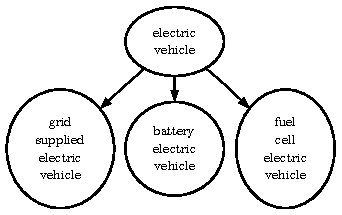
\includegraphics[width=0.45\textwidth]{images/OEOVehicles}}
    \subfigure[OEO electric vehicle commitments]{\label{oeoev:b}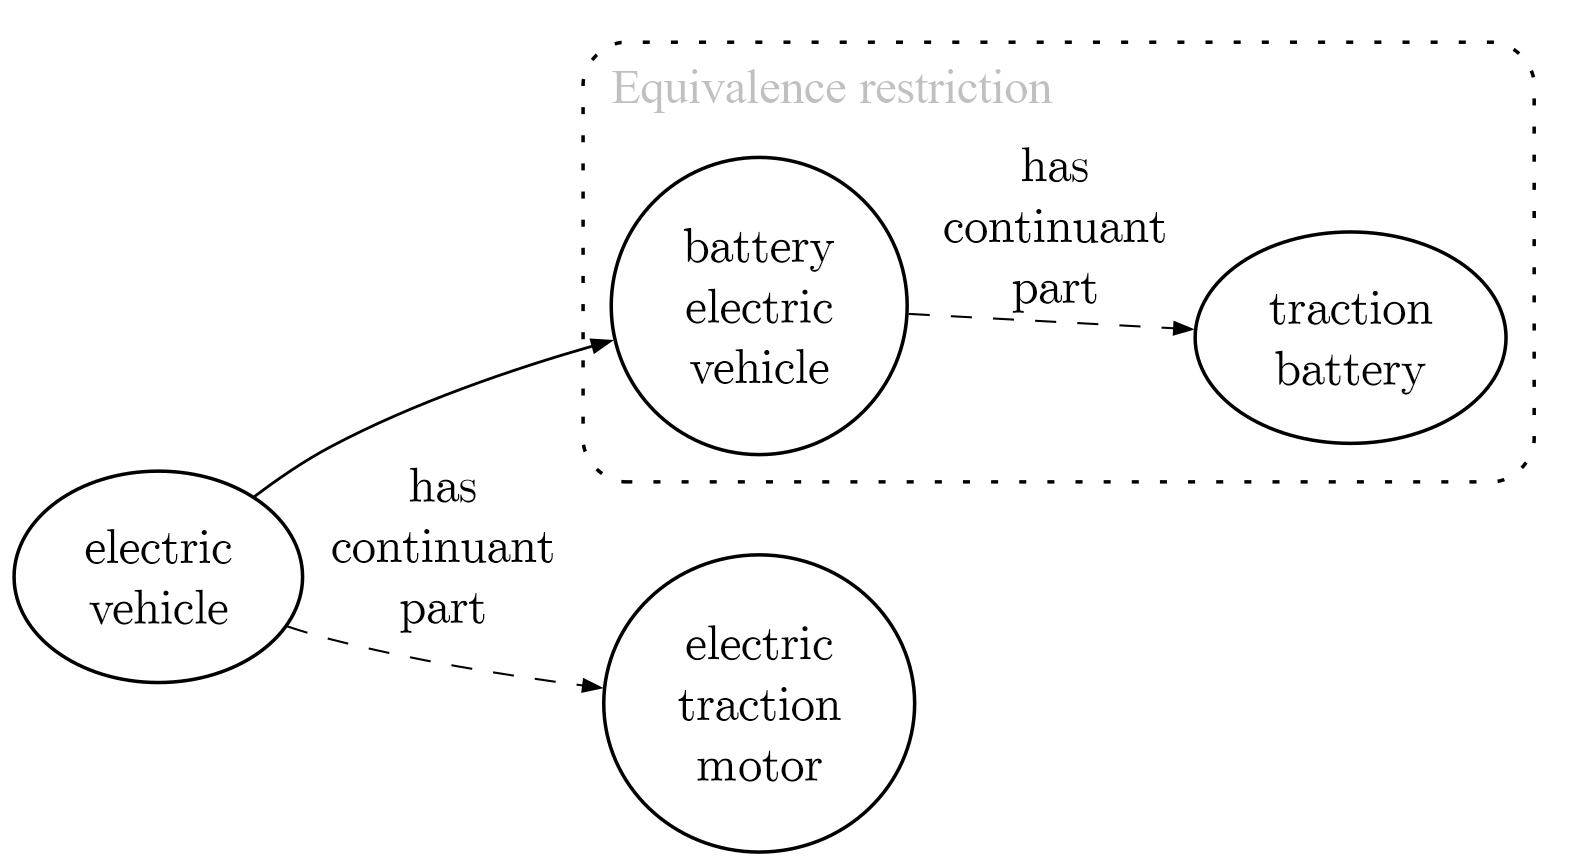
\includegraphics[width=0.45\textwidth]{images/OEOEV}}
    \caption{OEO ontological commitments relevant to the context of charging infrastructure. Note that we exclude grid related commitments, mostly because we have yet to define a scenario for that case.}
\end{figure}

\subsection{The Common Core Ontologies}

The CCO are 12 mid-level ontologies built as an extension of BFO and the
Relations Ontology (RO) intended to be used as a basis to model domains of
interest such as transportation infrastructure spacecrafts
\cite{Rudnicki.23September2020}. Like BFO, it is a realist ontology, which
means that it intends to model entities and data alike. The ontology avoids
being prescriptive, instead lets data modellers decide which asserted class
axioms are relevant for their particular applications. The ontology comes with
a guide that lets non ontology experts understand how to implement terms in the
ontology which is very helpful to involve domain experts of other fields in
ontology development.

We import a small subset of terms coming from these ontologies. Indeed, we
avoid importing whole ontologies by opting to do punctual extractions. This was
decided to avoid convolution of the final product, since we are expecting
developers to work with Protégé, if we imported all the classes they would have
a harder time finding where to place their new terms. We extract multiple
taxonomies and some axioms from these ontologies. These are listed during the
rest of this section.

\subsubsection{Vehicle taxonomy}

From the artifact ontology we extract terminology associated with vehicles. We
consider that their non-prescriptive approach offers a more manageable taxonomy
of vehicles that can be utilized across different fields of application. The
OEO classifies vehicles based on their energy consumption which is practical
for their applications but since we are not interested in non-electric vehicles
these become superfluous. Other reason to use the artifacts ontology
axiomatization is to profit from the other declarations coming from the same
suite of ontologies, particularly the axioms that allow `material artifacts'
with `sites' which will be helpful to handle concepts associated with parking.
The top upper levels of both taxonomies, besides both using BFO are slightly
different. The OEO classifies vehicles as artificial objects whereas the CCO as
`material artifacts'. The lower levels, despite being developed independently
are very similar, so similar  that they are practically already interoperable.
The taxonomies can be compared by looking at figures \ref{ccovectax} and
\ref{landvehicletaxoeo}.

\begin{figure}[h]
    \centering
    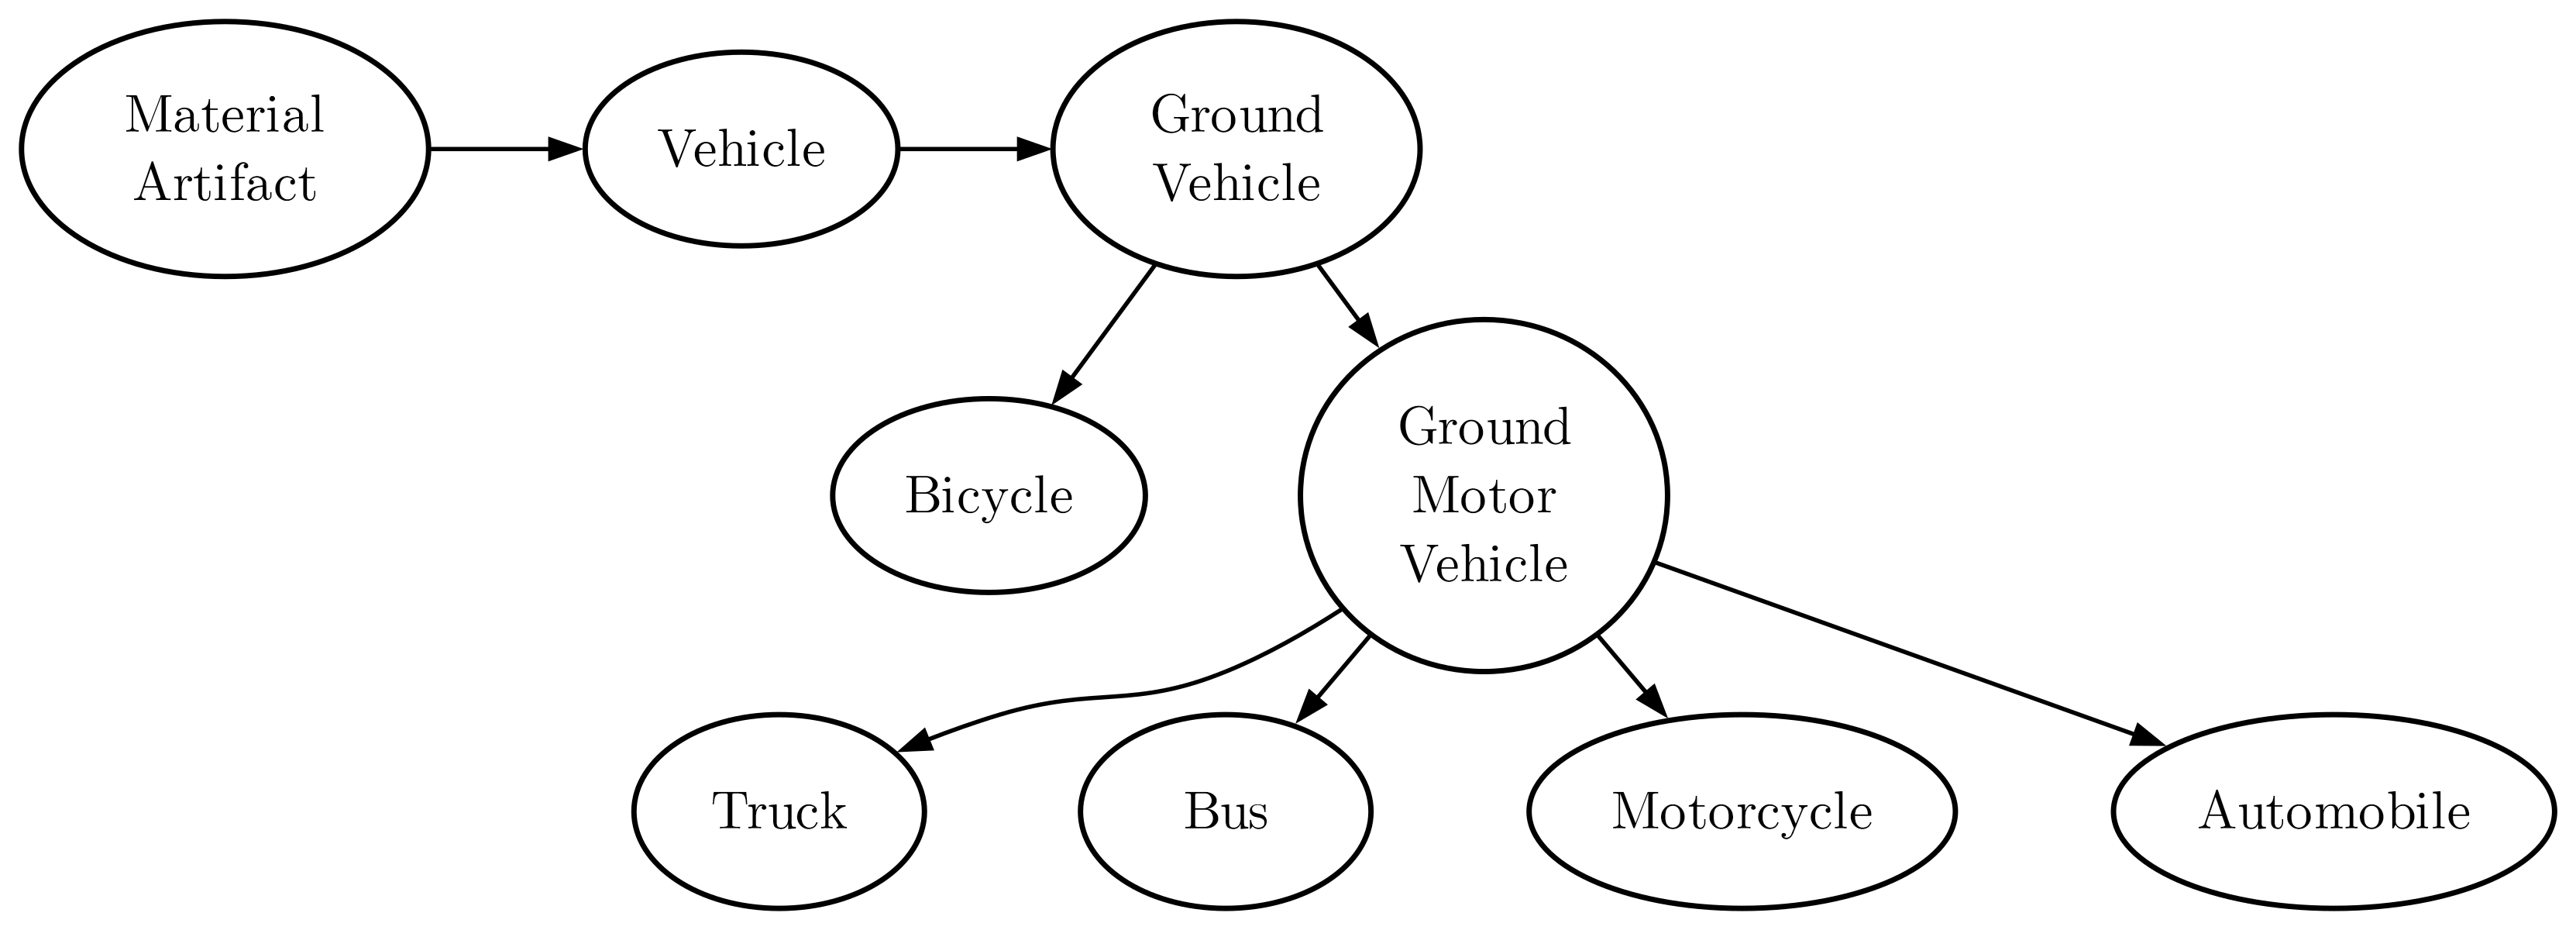
\includegraphics[width=0.9\textwidth]{images/CCOVehicles}
    \caption{The CCO vehicle taxonomy is slimmer and more streamlined to the concept of a vehicle.}
    \label{ccovectax}
\end{figure}
\begin{figure}[h]
    
    \centering
    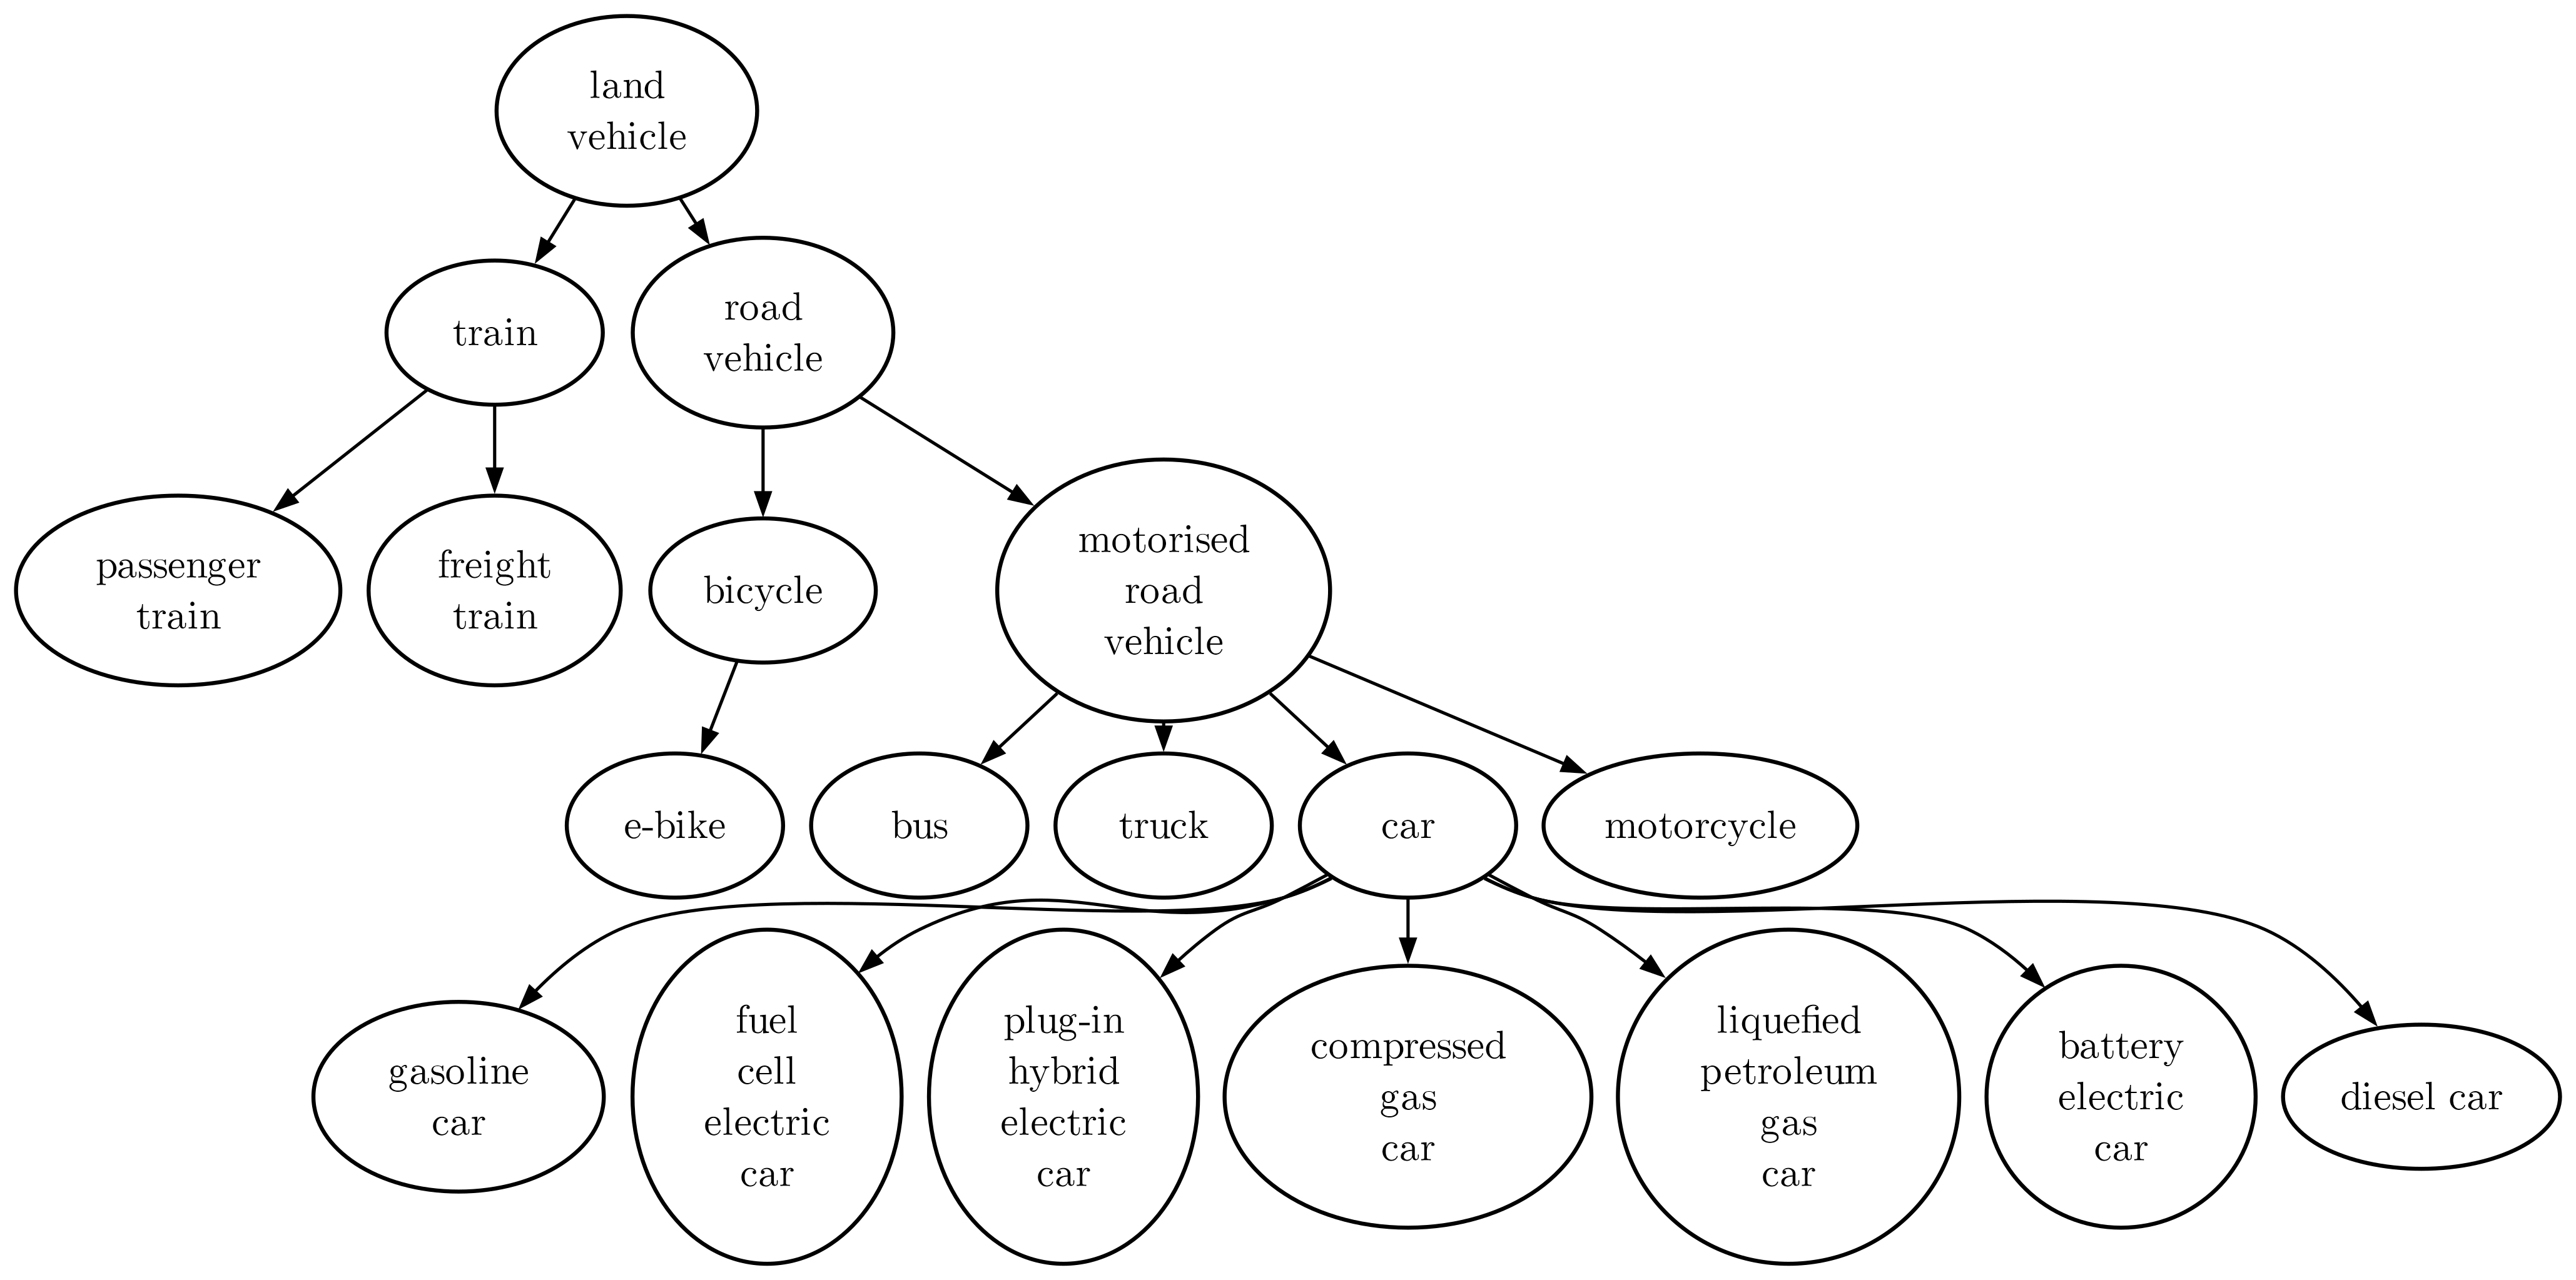
\includegraphics[width=0.9\textwidth]{images/OEOLVehicles}
    \caption{The OEO Land vehicle taxonomy is rich of axioms associated to the vehicles' energy consumption.}
    \label{landvehicletaxoeo}
\end{figure}

\subsubsection{Infrastructure}

The CCO offers a construct that aids to classify material artifacts as
infrastructure. It uses what in BFO are called `roles'. This allows arbitrary
assignment of the class. This is practical to us because charging stations in
reality are not always infrastructure, they are only in virtue of the agents
who assign them this role. In this sense a home wall box is not infrastructure
for a government agency but a public column is. Infrastructure rarely comes as
units but as  complex aggregates of artifacts, this is way we opt to import the
concept of infrastructure system. These axioms can be visualized in figure
\ref{infrastructurefigs}.

\begin{figure}[h]
    \centering
    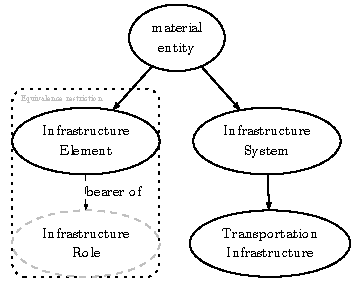
\includegraphics[width=0.8\textwidth]{images/infrastructureSystem}
    \caption{Common Core Ontologies infrastructure constraints.}
    \label{infrastructurefigs} 
\end{figure}

\subsubsection{Facilities}

As an only exception to our `scenario first' rule we import the facility
ontology to handle concepts like parking lots and dedicated charging stations.
An alternative would be to stick to using material entities, but we consider
this differentiation practical in the long run. Specially when considering
interoperability with future transportation research ontologies


\subsection{iCity Parking ontology}

The TPSO has a module for terminology associated with parking which provides
concepts like parking spaces, areas and fees. It also offers definitions for
charging stations, but these are too shallow for our applications as they are
at most features of parking spaces. The subclassification of charging stations
are `standard', `medium' and `fast' which are defined based on the definitions
of the Environmental Protection Department whose source was not explicitly
pointed. If having such a classification is meaningful to our applications is
yet to be defined. The TPSO has its own upper level ontology modules which
supply axiom definitions for change, mereology and time. These modules are
fundamentally incompatible with the BFO. The Change module of the ontology
relies on the utilization of a 4 dimensional approach to model time changing
concepts. This means that every object has a perdurant and its manifestations
bear their changes. Since we are not intending to axiomatize time relations in
OWL and instead opt to delegate that to data modellers we opt not to share that
approach. All the axioms that are interesting to us from the Parking ontology
can be visualized in figure \ref{parkingfig}. BFO has its own approach to
handle descriptions of change, this will be addressed in its respective
section.

\begin{figure}[h]
    \centering
    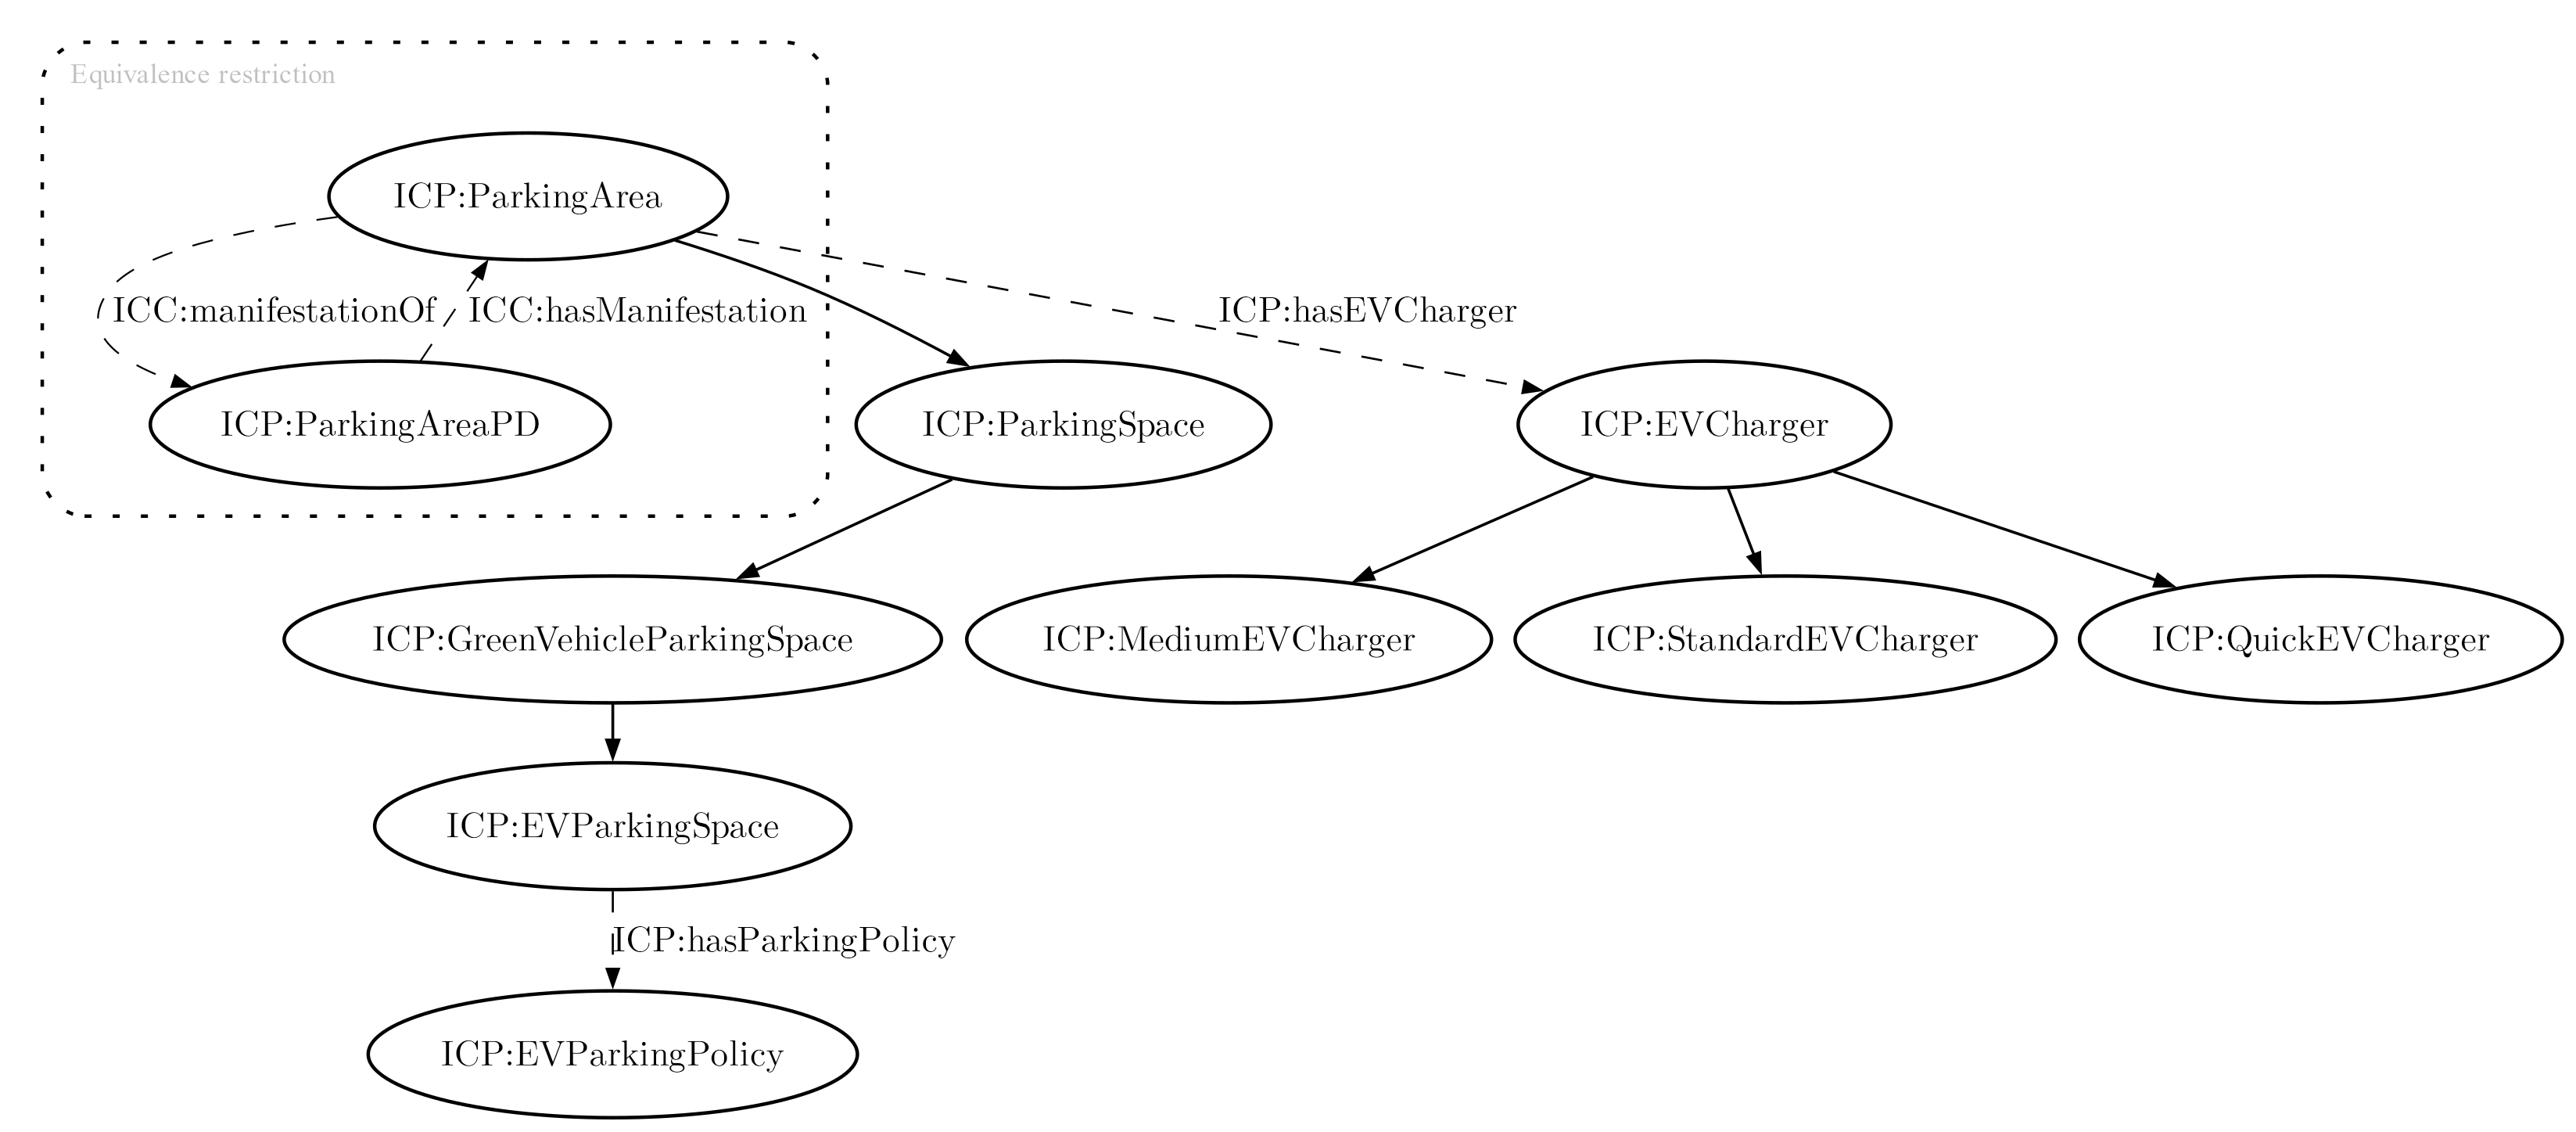
\includegraphics[width=1.0\textwidth]{images/PARKING}
    \caption{iCity parking ontology commitments associated to charging infrastructure.}
    \label{parkingfig}
\end{figure}

\subsubsection{The Basic Formal Ontology}
\label{upperlevel}

Top-level ontologies or foundational ontologies intend to model domain neutral
categories and relations \cite{Arp.2015}. These are not a hard requirement to
build an ontology but can make the difference regarding its interoperability.
Choosing (or developing) a top-level ontology is not an easy task because a
modeller needs to have a deep understanding of their domain and the possible
applications. In 2022 a special issue of applied ontology \cite{Borgo.2022}
allowed ontology developers to exemplify the usage of multiple prominent
top-level ontologies. In theory, we would select our ontology by following the
motivating scenarios defined in section \ref{methodology}. But since we are
intending to build on the efforts from the OEO we streamlined to using BFO.
This decision comes not without compromises. 

BFO sacrifices expressivity for a simpler modelling intuition. It has
weaknesses in the field of modal propositions which are prominent in both
transportation research en energy systems analysis, particularly in the context
of forecasts and simulation\footnote{However this weakness is addressed by CCO
with their ModalRelationOntology which we consider importing. }. Unlike the
TPSO foundational modules, BFO delegates its time indexing to the applications
by keeping it outside the OWL implementation. BFO has a rather simple initial
learning curve that can be used to facilitate the inclusion of new developers.
But still becomes very steep when dealing some of its more complex terms (i.e.
`process profile', `disposition' vs `quality'), this can lead to frustrations
or miss-uses.

There are some important features of BFO that we intend to take advantage of.
The first is that it allows the existence of `sites' in the same dimension as
`material entities'. This is because charging events depend on the dynamics of
vehicles being present and absent. We also need it to characterize the
mereotopology of charging stations. A second important feature are `process
profiles', since we consider that the charging event can have multiple
dimensions that can describe it that have to be associated with each other.
Using those we can describe events in virtue of their occupancy, power rates
and energy transfers.


\section{Methodology}
\label{methodology}
\section{Results}
\label{results}

At the time of this publication the ontology has an open git
repository\footnote{Note for the editors: The publishing of the repository is
being subject to export control, we would update the links accordingly in the
camera-ready version. }. This repository has developer documentation where the
motivating scenarios along with their competency questions are written. A quick
introduction for developers is also part of this documentation. This
documentation is written using exclusively markdown files which can be rendered
into webpages with different packages, we opt for using
MkDocs\footnote{https://www.mkdocs.org/} because of its simplicity. For the
ontology documentation and the IRI resolution, we are still exploring solutions.
We are tending towards Widoco\footnote{https://github.com/dgarijo/Widoco}.

We implemented a Python test suite that allows the incremental development of
the ontology using competency questions. This suite classifies the queries into
two types. Those who act on classes (TBox) like \hyperref[CQ1.1]{CQ 1.1} and
those that act on individuals (ABox) like \hyperref[CQ2.0]{CQ 2.0}. To handle
the ABox queries we rewrite the natural language questions as ASK queries in
SPARQL  that returns either true or false values. We also declare a model in
Turtle Syntax that instantiates the referred classes. For example
\hyperref[CQ2.0]{CQ 2.0} is written as listing \ref{lst:1} and its corresponding
model \ref{lst:2} populates the ABox. The TBox questions are evaluated by
checking entailment using DL queries such as the one in listing \ref{lst:3}
which corresponds to \hyperref[CQ1.1]{CQ 1.1}.

\begin{listing}[h]
    
    \begin{minted}[fontsize=\small]{sparql}
        ASK WHERE {
            SELECT (COUNT(?parkingSpaces) AS ?vehicleCapacity)  
            WHERE  {  :SomeParkingArea obo:BFO_0000178 ?parkingSpaces . 
                      ?parkingSpaces rdf:type chio:CHIO_00000002 . }
            HAVING ( ?vehicleCapacity = 2 ) }
    \end{minted}
    \caption{Example ABox query. (Given a parking area with two parking places) What is the (vehicle) capacity of parking lot P? (2). The namespaces are omitted.}
    \label{lst:1}
\end{listing}

\begin{listing}[h]
    \begin{minted}[fontsize=\small]{turtle}
        :SomeParkingSpaceA a chio:CHIO_00000002 .
        :SomeParkingSpaceB a chio:CHIO_00000002 .
        :SomeParkingArea a chio:CHIO_00000001 ;
                         obo:BFO_0000178 :SomeParkingSpaceA,
                                         :SomeParkingSpaceB .
    \end{minted}
    \caption{Example ABox instances. Two charging spaces (that can hold at most one car at a time) are part of some parking area. Namespace prefixes are omitted, the chio namespace refers to the charging ontology.}
    \label{lst:2}
\end{listing}

\begin{listing}[h]
    \begin{minted}[fontsize=\small]{text}
        'charging station' SubClassOf 'parking facility' 
            and 'has continuant part' some 'charging column'
    \end{minted}
    \caption{Example DL Query used to evaluate TBox competency. A charging station is a kind of parking facility and has charging columns as parts.}
    \label{lst:3}
\end{listing}

Since we aim for a high rate of reusability, most of the efforts have been aimed
towards finding concepts from existing ontologies. We import the entire CCO
version of the BFO which already includes basic RO axioms. We import the
excerpts from OEO and CCO mentioned in section \ref{methodology}, we do this by
providing scripts that ensure transparency and reproducibility. These scripts
point to specific versions of the ontologies that can be updated based on
developing needs. In some cases, we reimplemented terms and pointed out the ones
from other ontologies by using mappings. This was the case for the axioms from
the TPSO Parking Ontology (figure \ref{parkingfig}). Our interpretation of
parking areas and spaces is similar, but we rely on the mereology of BFO.
Instead of assigning the charging stations to parking spaces directly we opt to
use the facility axioms from CCO. These implementations can be visualized in
figure \ref{parkingchio}.

\begin{figure}[h]
    \centering
    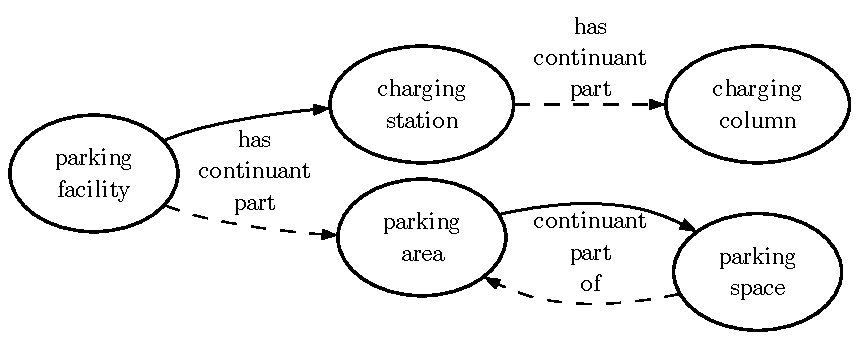
\includegraphics{images/CHIOParking.pdf}
    \caption{Parking area, place, and facility implementations in our ontology. This model builds on the taxonomy of the CCO Facility Ontology. Solid arrows represent super-class relations.}
    \label{parkingchio}
\end{figure}



    
\section{Conclusion}
\label{conclusion}

Questions on electrification of the transport sector and other research trends
have as ultimate goal to put a stop to climate-change driving carbon emissions.
These study fields deal with complex systems whose boundaries tend to differ
based on the research questions themselves. These differences become troublesome
when exchanging data because, in most cases, the person producing it is not
always available to clarify misunderstandings. Metadata improves this situation
significantly, but their content is also subject to interpretation. While
ontologies can't solve problems of ambiguity, they can ease them by offering a
way of explicitly declare semantics. With this small ontology project we intend
to offer a reference point for communication not only between transport and
energy researchers but also any person whose work involves electric vehicle
charging stations which are components of larger infrastructure systems. The
ontology development is streamlined thanks to the preparation effort that we
invested. We consider that the methodology we used to prepare the environment
can be re-utilized for other ontologies. In fact an important part was taken
already from what we learned from the OEO development. In further works we
expect to use our approach to create, map and expand ontologies usable for
transportation research and cover other niches that are out of scope of the OEO.

% \begin{acknowledgments}
Some Acknowledgements
\end{acknowledgments}

%% Define the bibliography file to be used
\bibliography{bibliography}

%%
%% If your work has an appendix, this is the place to put it.
\newpage
\appendix



\end{document}

%%
%% End of file
